\section{\npsel pre-selection}
\label{app:nuepresel}

Figures~\ref{fig:1eNp:dataMCRun1:reco_nu_vtx}-\ref{fig:1eNp:dataMCRun1:pi02} show the data-MC comparison for all \npsel variables in Run1 + Run3 open data after \npsel preselection.

\begin{figure}[H] 
\begin{center}
    \begin{subfigure}[b]{0.3\textwidth}
    \centering
    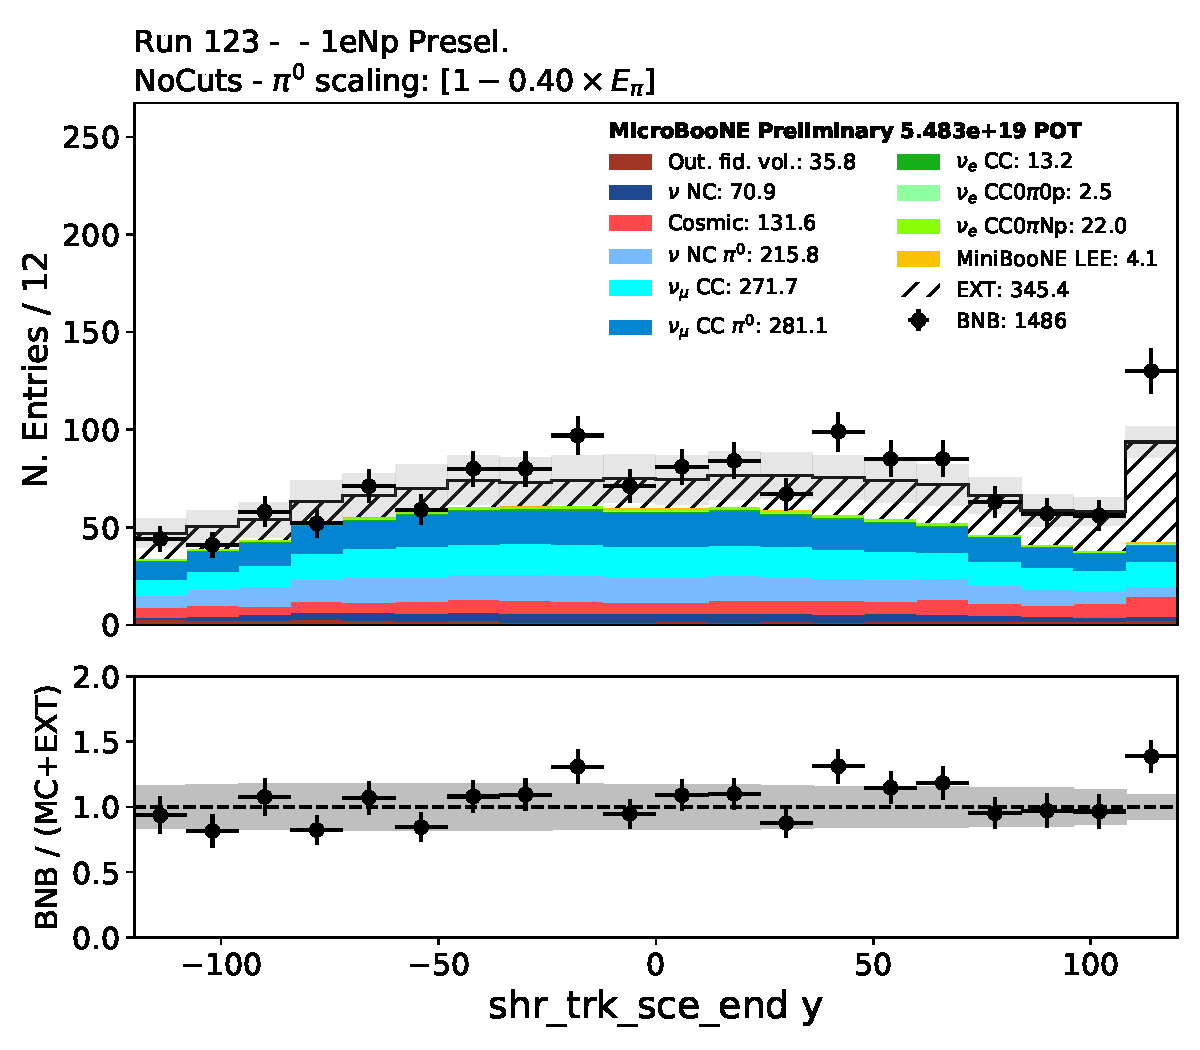
\includegraphics[width=1.00\textwidth]{1eNp/dataMCRun13/shr_trk_sce_end_y.pdf}
    \caption{\label{fig:1eNp:dataMCRun1:shr_trk_sce_end_y} shr\_trk\_sce\_end\_y }
    \end{subfigure}
    \begin{subfigure}[b]{0.3\textwidth}
    \centering
    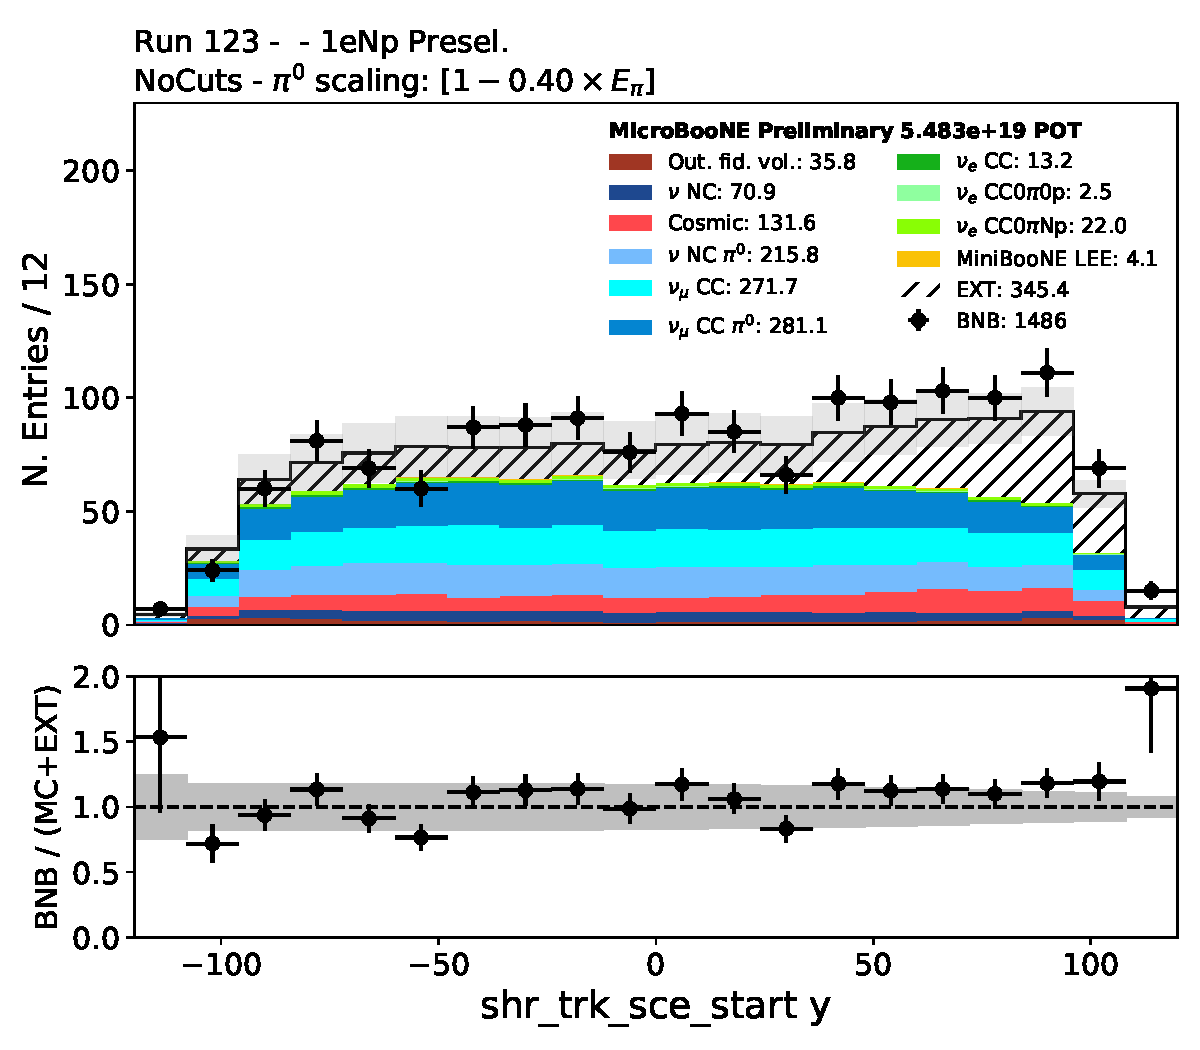
\includegraphics[width=1.00\textwidth]{1eNp/dataMCRun13/shr_trk_sce_start_y.pdf}
    \caption{\label{fig:1eNp:dataMCRun1:shr_trk_sce_start_y} shr\_trk\_sce\_start\_y}
    \end{subfigure}
\caption{\label{fig:1eNp:dataMCRun1:reco_nu_vtx}Data-MC comparison in the Run1 open data after the \npsel preselection.}
\end{center}
\end{figure}

\begin{figure}[H] 
\begin{center}
    \begin{subfigure}[b]{0.3\textwidth}
    \centering
    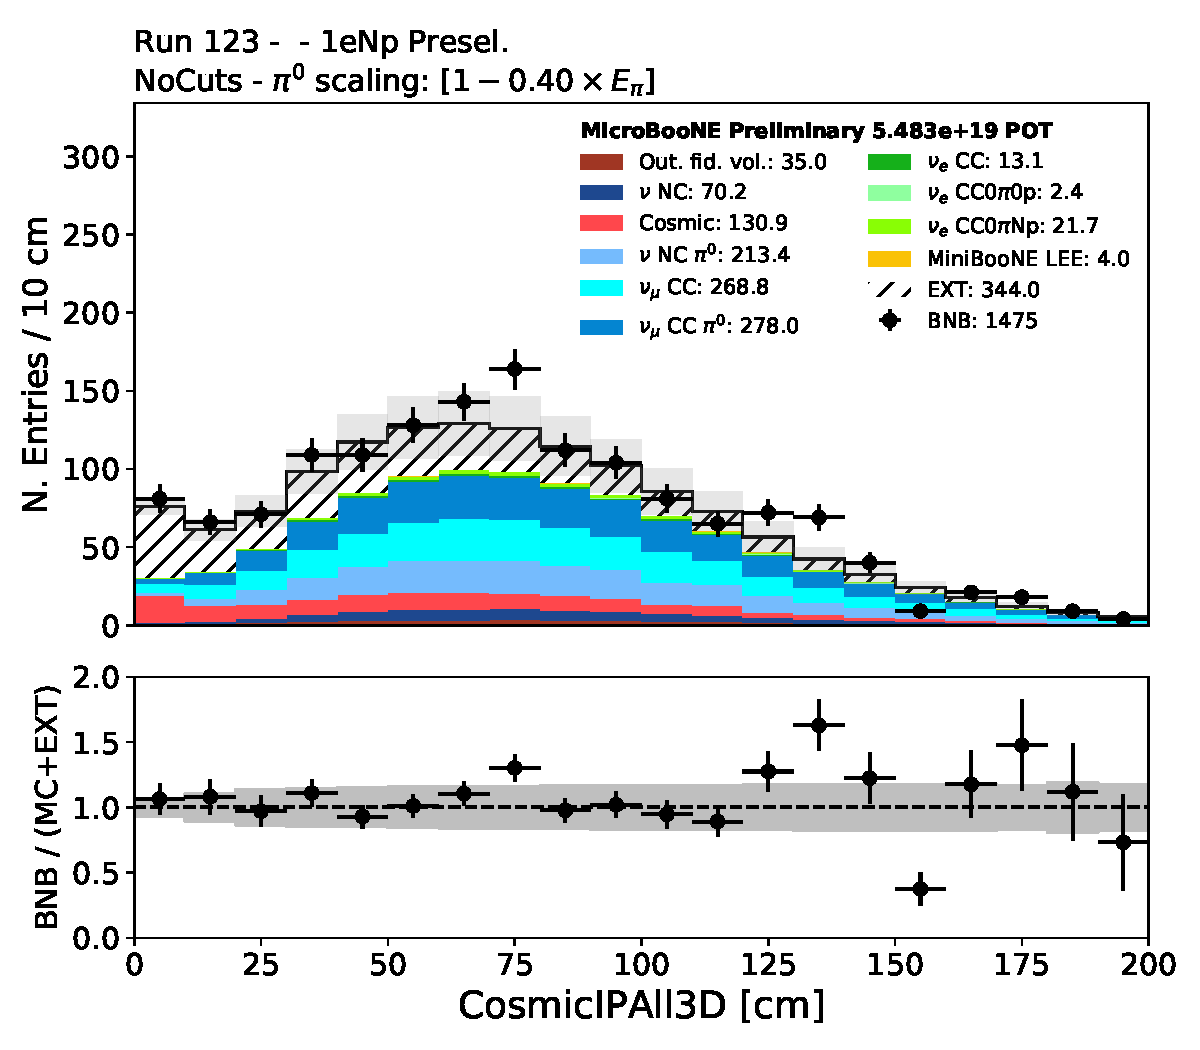
\includegraphics[width=1.00\textwidth]{1eNp/dataMCRun13/CosmicIPAll3D.pdf}
    \caption{\label{fig:1eNp:dataMCRun1:CosmicIP} CosmicIP3D }
    \end{subfigure}
    \begin{subfigure}[b]{0.3\textwidth}
    \centering
    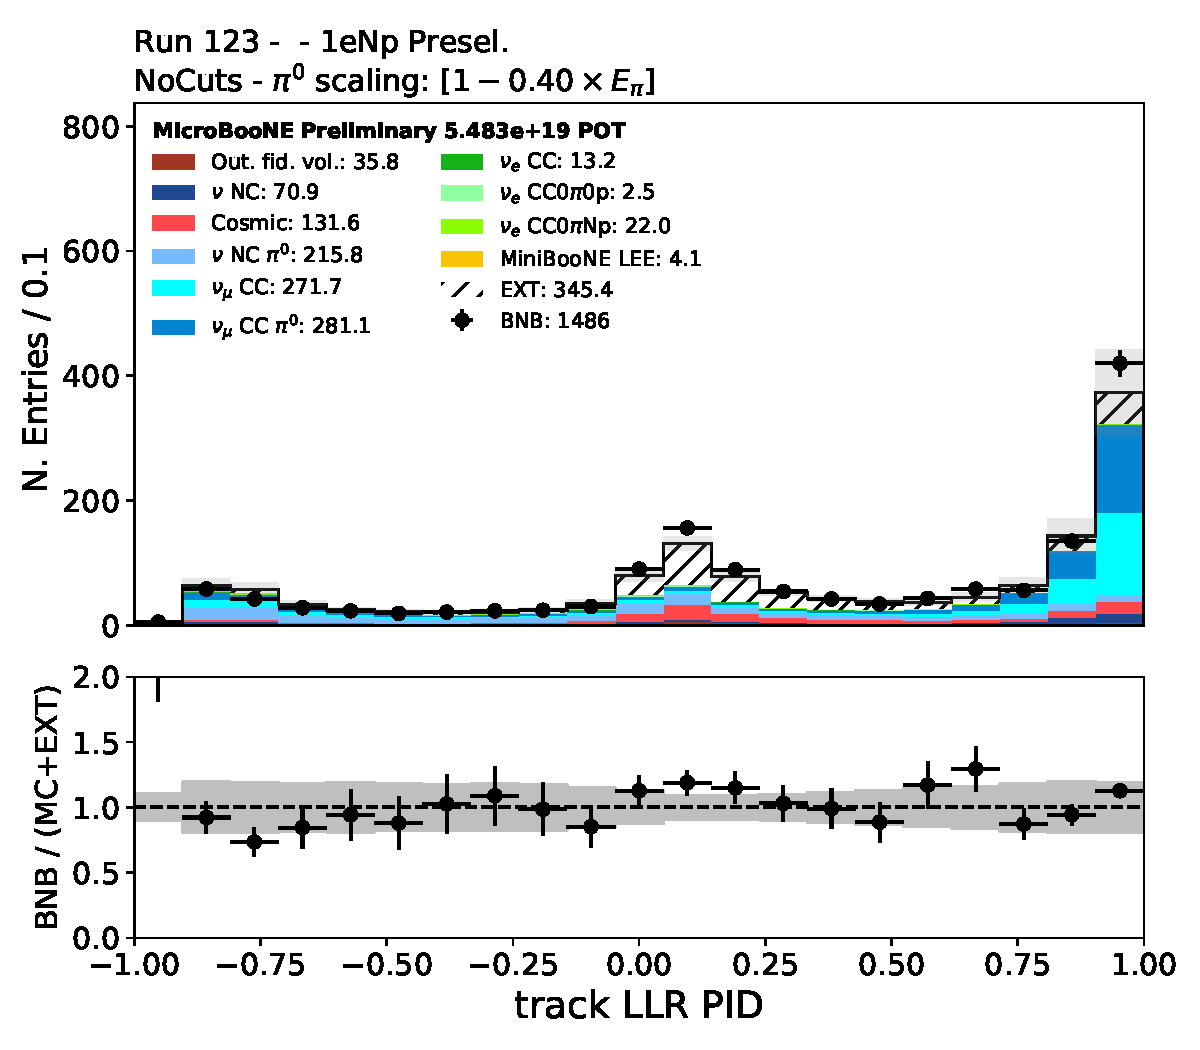
\includegraphics[width=1.00\textwidth]{1eNp/dataMCRun13/trkpid.pdf}
    \caption{\label{fig:1eNp:dataMCRun1:trkpid} trkpid }
    \end{subfigure}
    \begin{subfigure}[b]{0.3\textwidth}
    \centering
    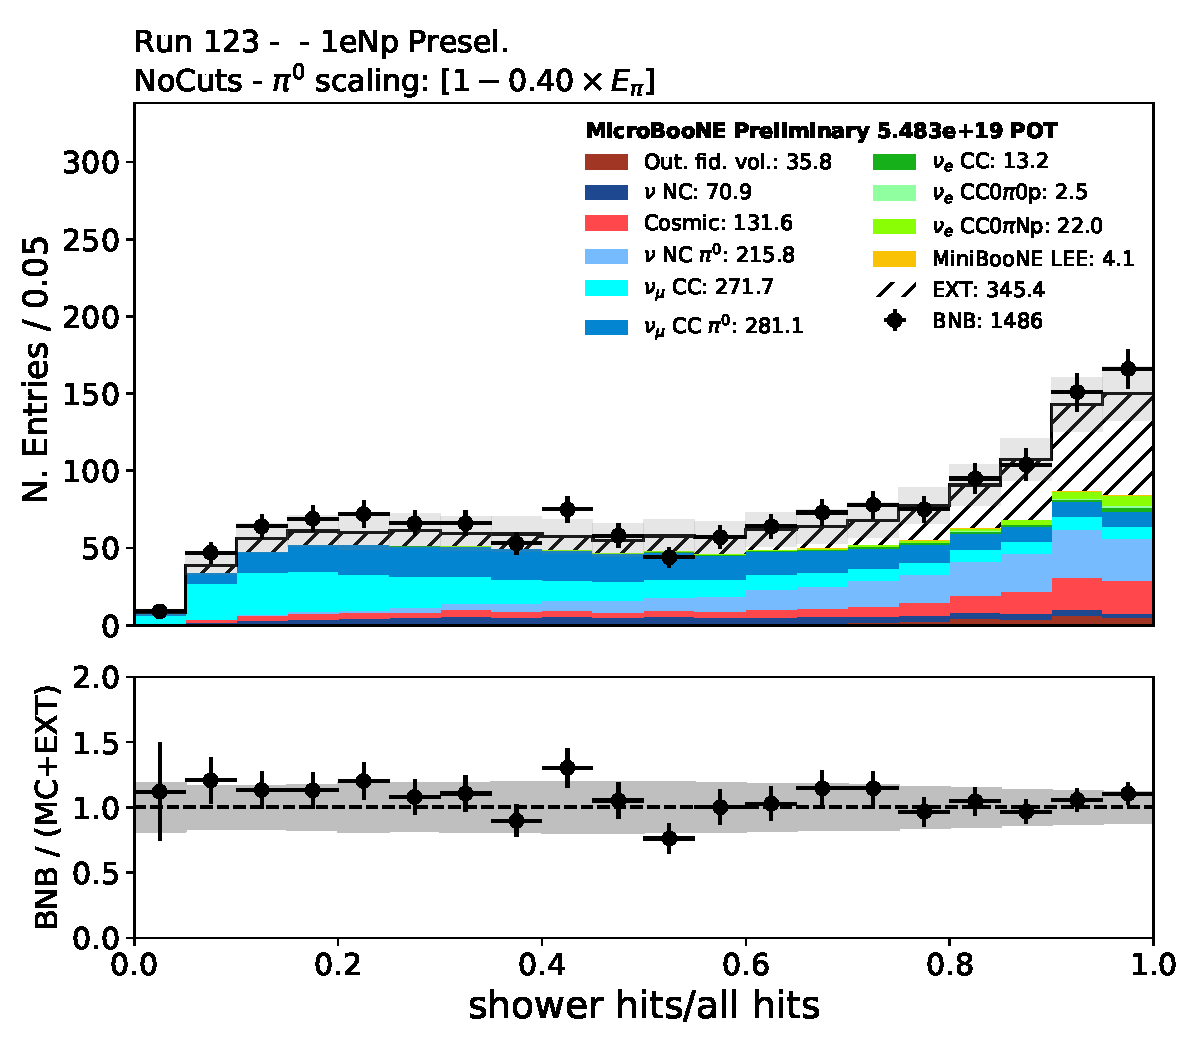
\includegraphics[width=1.00\textwidth]{1eNp/dataMCRun13/hits_ratio.pdf}
    \caption{\label{fig:1eNp:dataMCRun1:hits_ratio} hits\_ratio }
    \end{subfigure}
\caption{\label{fig:1eNp:dataMCRun1:cosmic}Data-MC comparison in the Run1 open data after the \npsel preselection.}
\end{center}
\end{figure}

\begin{figure}[H] 
\begin{center}
    \begin{subfigure}[b]{0.3\textwidth}
    \centering
    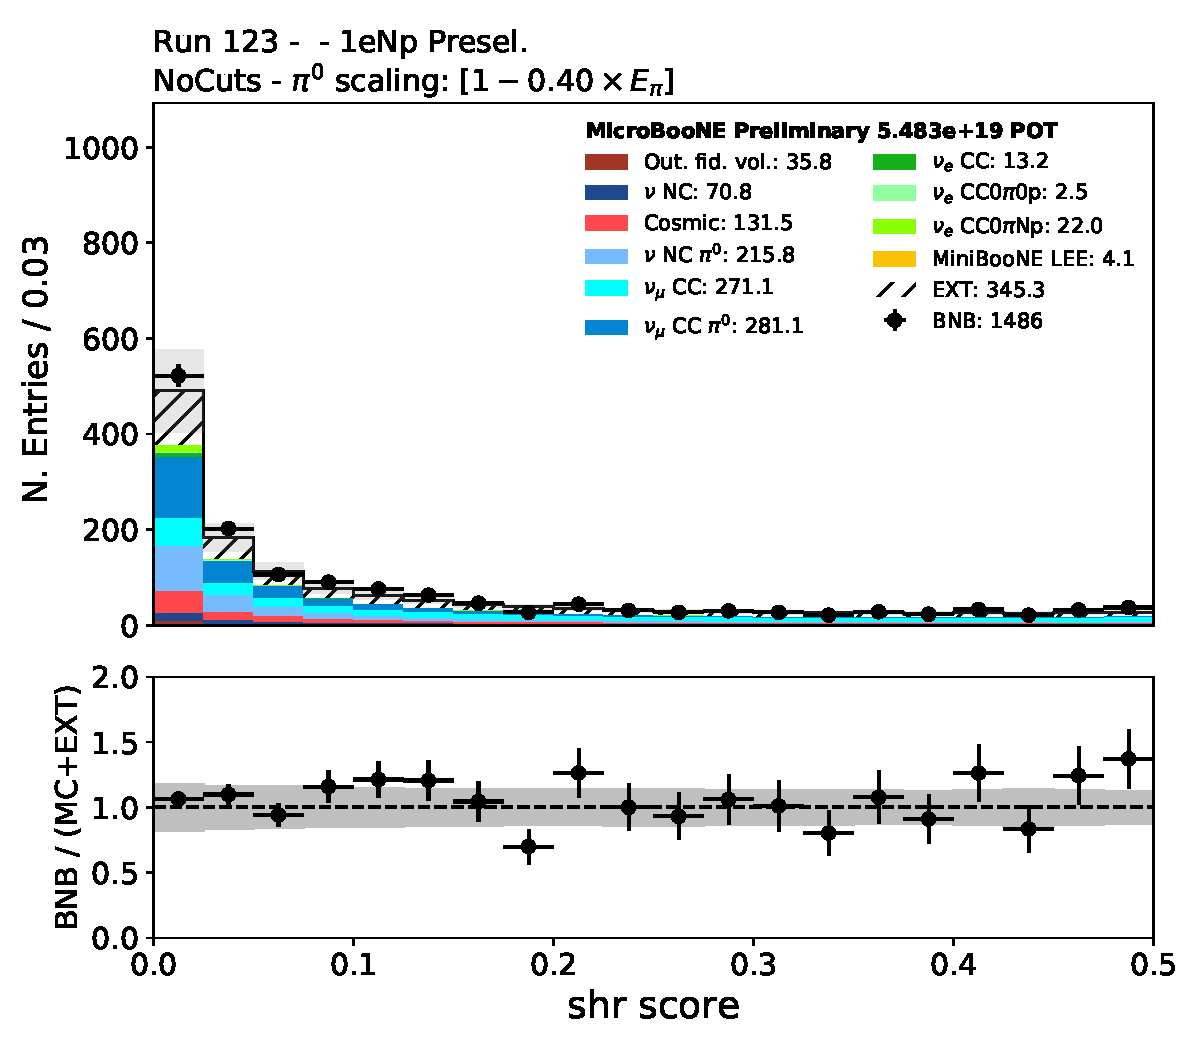
\includegraphics[width=1.00\textwidth]{1eNp/dataMCRun13/shr_score.pdf}
    \caption{\label{fig:1eNp:dataMCRun1:shr_score} shr\_score }
    \end{subfigure}
    \begin{subfigure}[b]{0.3\textwidth}
    \centering
    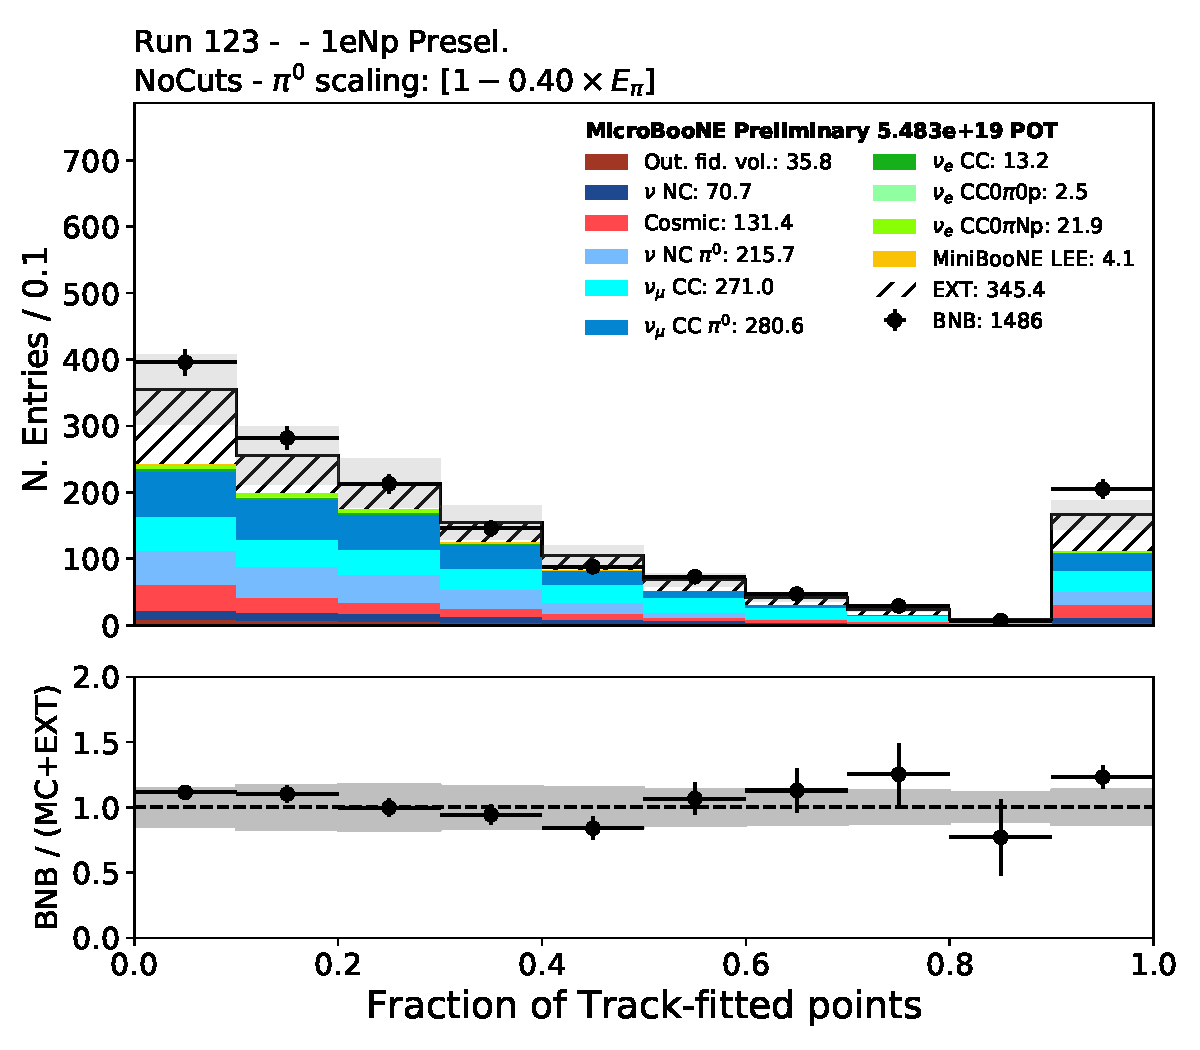
\includegraphics[width=1.00\textwidth]{1eNp/dataMCRun13/trkfit.pdf}
    \caption{\label{fig:1eNp:dataMCRun1:trkfit} trkfit }
    \end{subfigure}
    \begin{subfigure}[b]{0.3\textwidth}
    \centering
    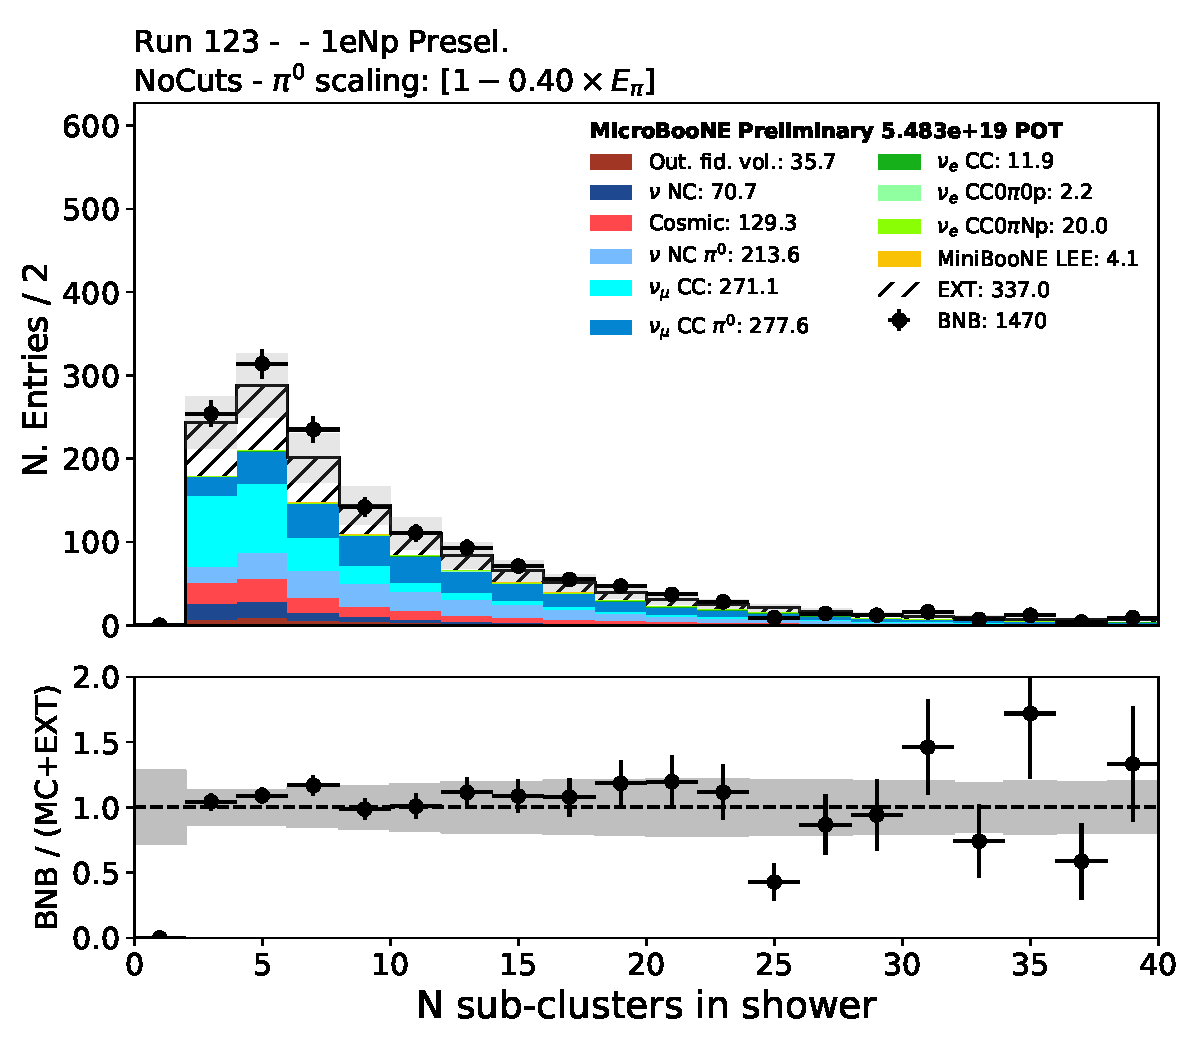
\includegraphics[width=1.00\textwidth]{1eNp/dataMCRun13/subcluster.pdf}
    \caption{\label{fig:1eNp:dataMCRun1:subcluster} subcluster }
    \end{subfigure}
\caption{\label{fig:1eNp:dataMCRun1:numu1}Data-MC comparison in the Run1 open data after the \npsel preselection.}
\end{center}
\end{figure}

\begin{figure}[H] 
\begin{center}
    \begin{subfigure}[b]{0.3\textwidth}
    \centering
    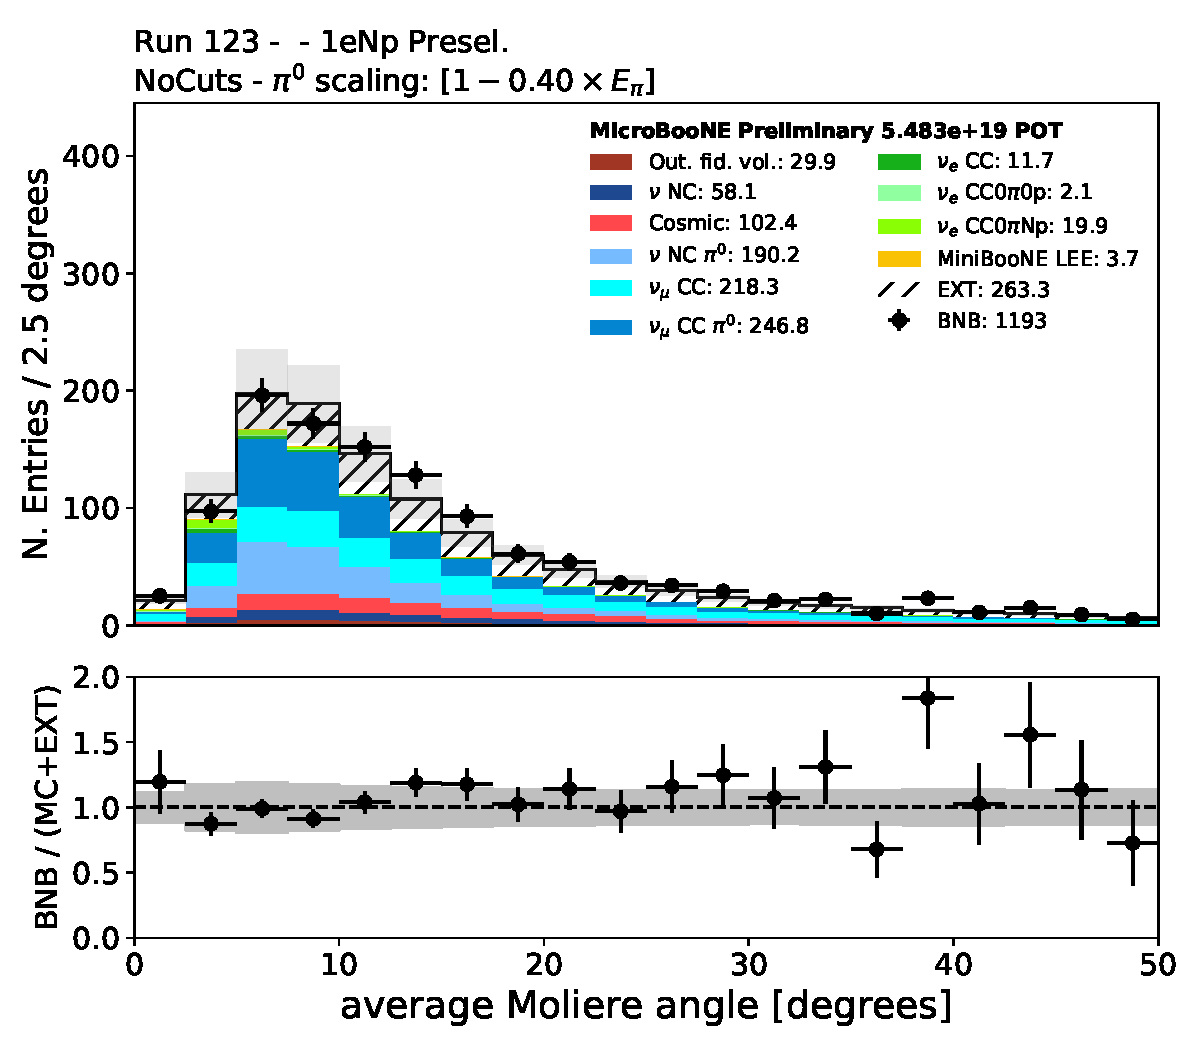
\includegraphics[width=1.00\textwidth]{1eNp/dataMCRun13/shrmoliereavg.pdf}
    \caption{\label{fig:1eNp:dataMCRun1:shrmoliereavg} shrmoliereavg }
    \end{subfigure}
    \begin{subfigure}[b]{0.3\textwidth}
    \centering
    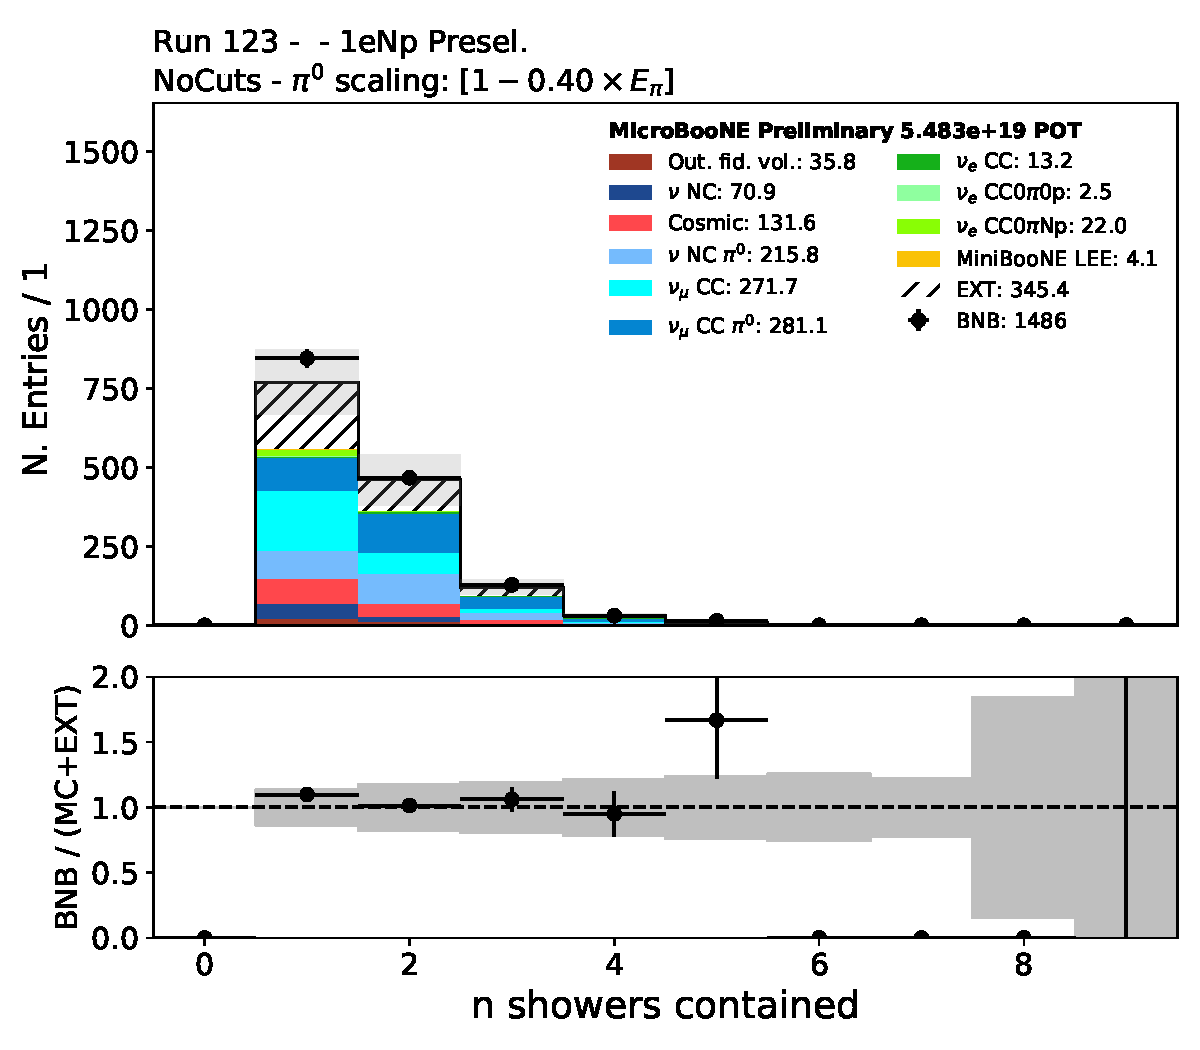
\includegraphics[width=1.00\textwidth]{1eNp/dataMCRun13/n_showers_contained.pdf}
    \caption{\label{fig:1eNp:dataMCRun1:n_showers_contained} n\_showers\_contained }
    \end{subfigure}
    \begin{subfigure}[b]{0.3\textwidth}
    \centering
    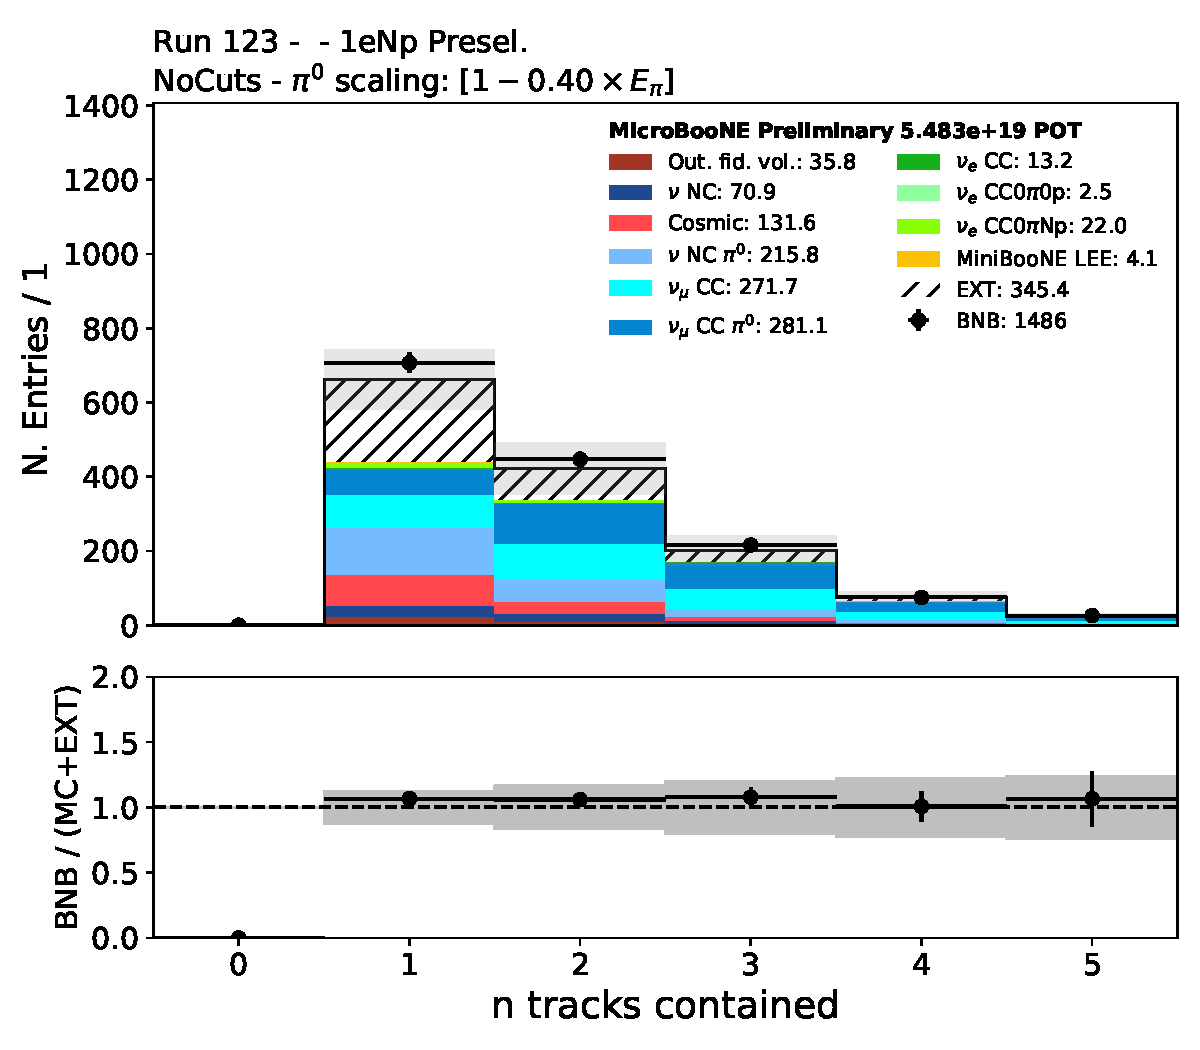
\includegraphics[width=1.00\textwidth]{1eNp/dataMCRun13/n_tracks_contained.pdf}
    \caption{\label{fig:1eNp:dataMCRun1:n_tracks_contained} n\_tracks\_contained }
    \end{subfigure}
\caption{\label{fig:1eNp:dataMCRun1:numu2}Data-MC comparison in the Run1 open data after the \npsel preselection.}
\end{center}
\end{figure}

\begin{figure}[H] 
\begin{center}
    \begin{subfigure}[b]{0.3\textwidth}
    \centering
    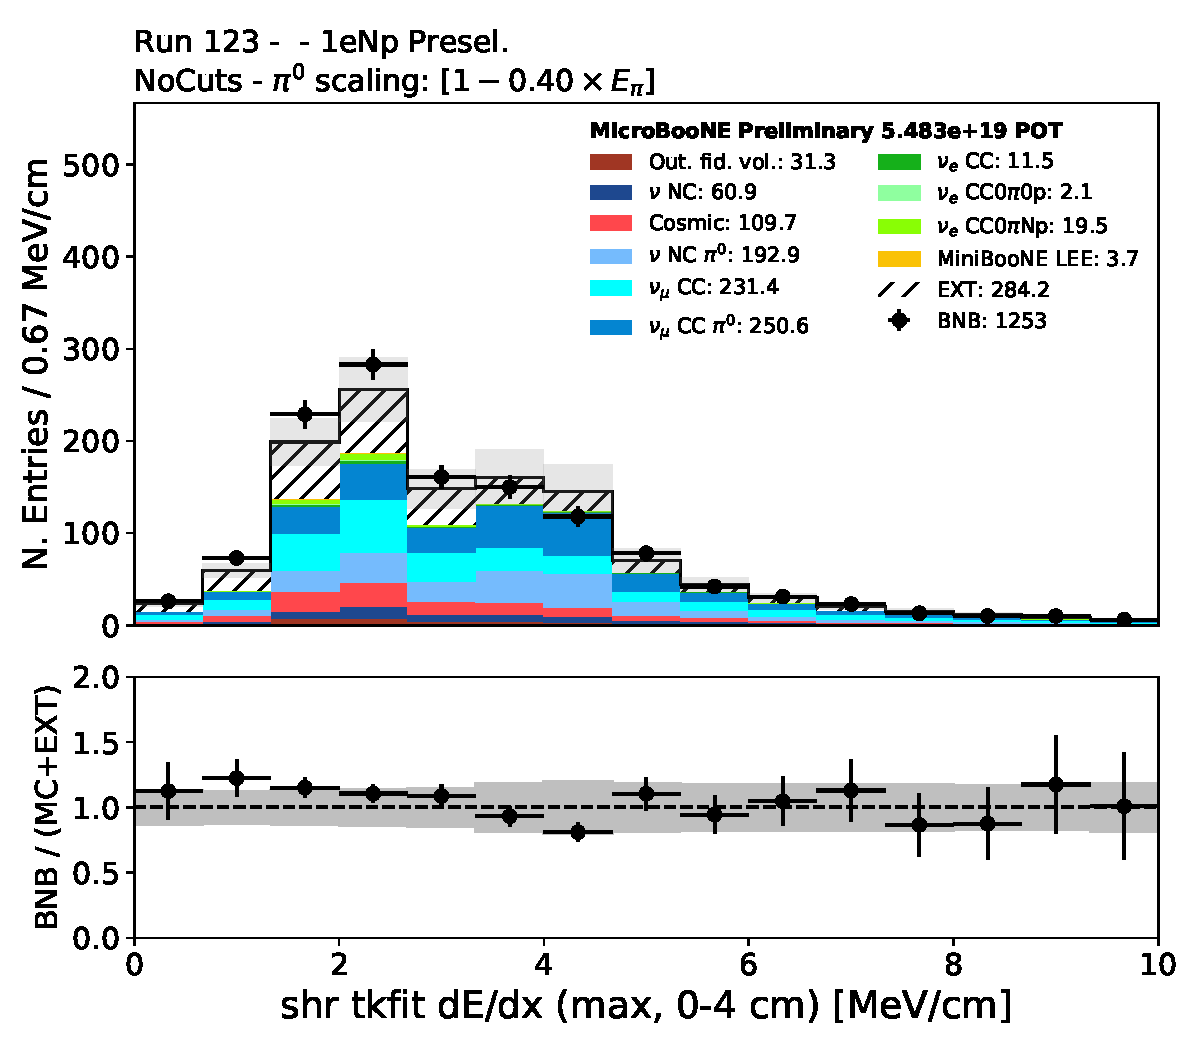
\includegraphics[width=1.00\textwidth]{1eNp/dataMCRun13/shr_tkfit_dedx_max.pdf}
    \caption{\label{fig:1eNp:dataMCRun1:shr_tkfit_dedx_max} shr\_tkfit\_dedx\_max }
    \end{subfigure}
        \begin{subfigure}[b]{0.3\textwidth}
    \centering
    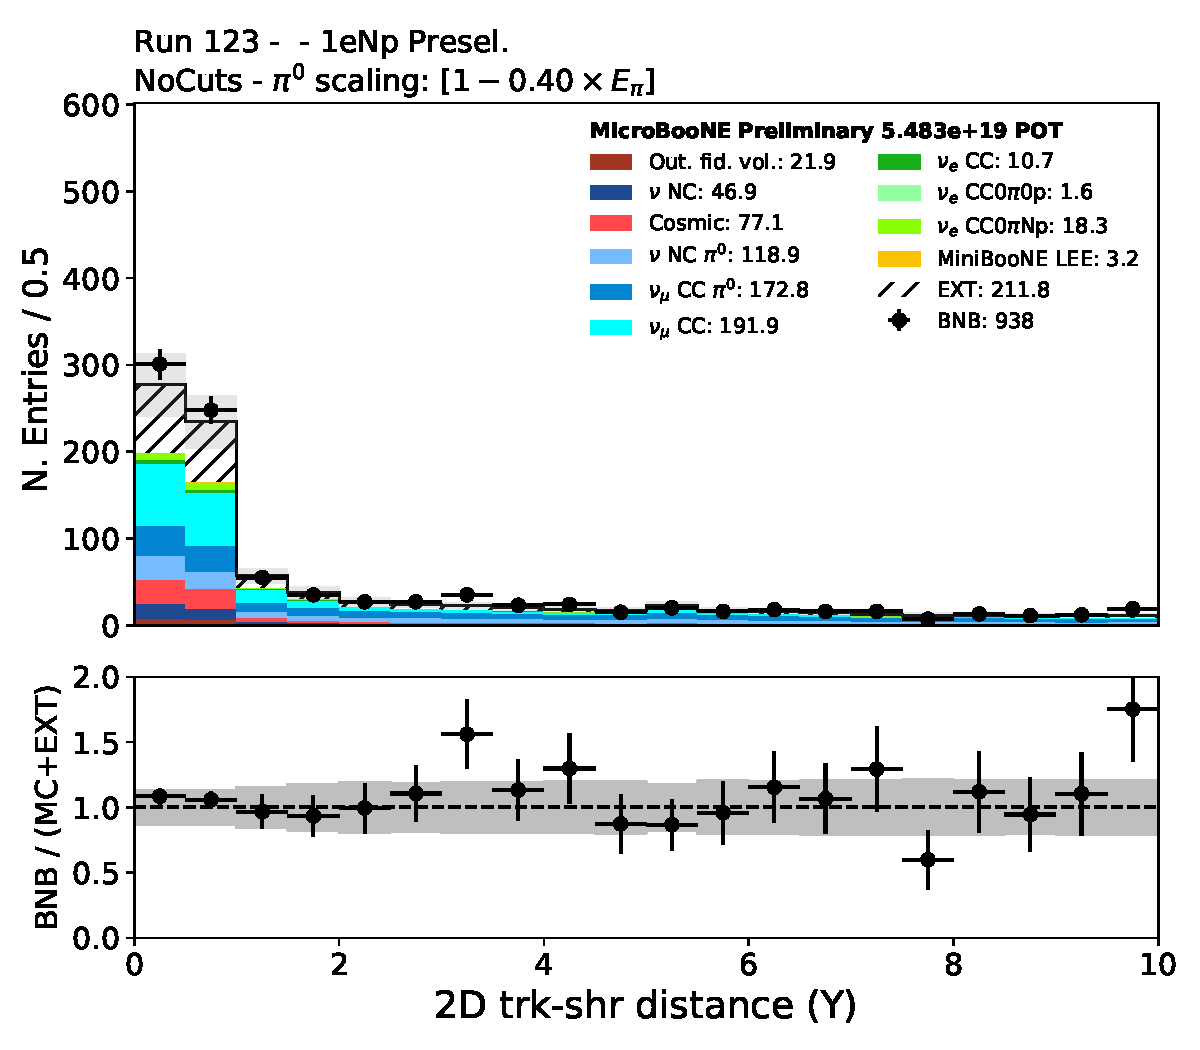
\includegraphics[width=1.00\textwidth]{1eNp/dataMCRun13/trkshrhitdist2.pdf}
    \caption{\label{fig:1eNp:dataMCRun1:trkshrhitdist2} trkshrhitdist2 }
    \end{subfigure}
\caption{\label{fig:1eNp:dataMCRun1:shr_tkfit_dedx}Data-MC comparison in the Run1 open data after the \npsel preselection.}
\end{center}
\end{figure}

\begin{figure}[H] 
\begin{center}
    \begin{subfigure}[b]{0.3\textwidth}
    \centering
    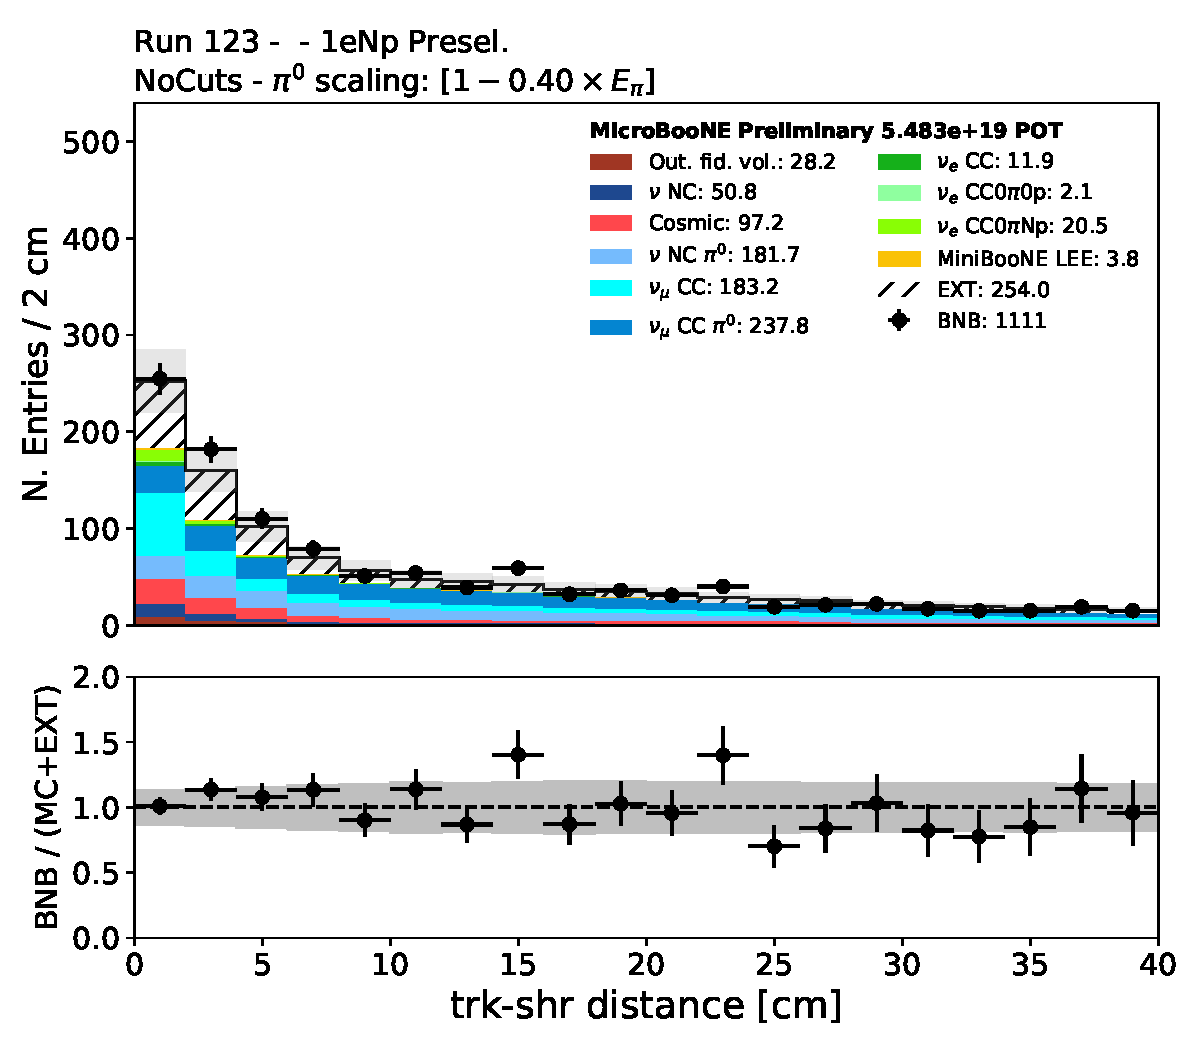
\includegraphics[width=1.00\textwidth]{1eNp/dataMCRun13/tksh_distance.pdf}
    \caption{\label{fig:1eNp:dataMCRun1:tksh_distance} tksh\_distance }
    \end{subfigure}
    \begin{subfigure}[b]{0.3\textwidth}
    \centering
    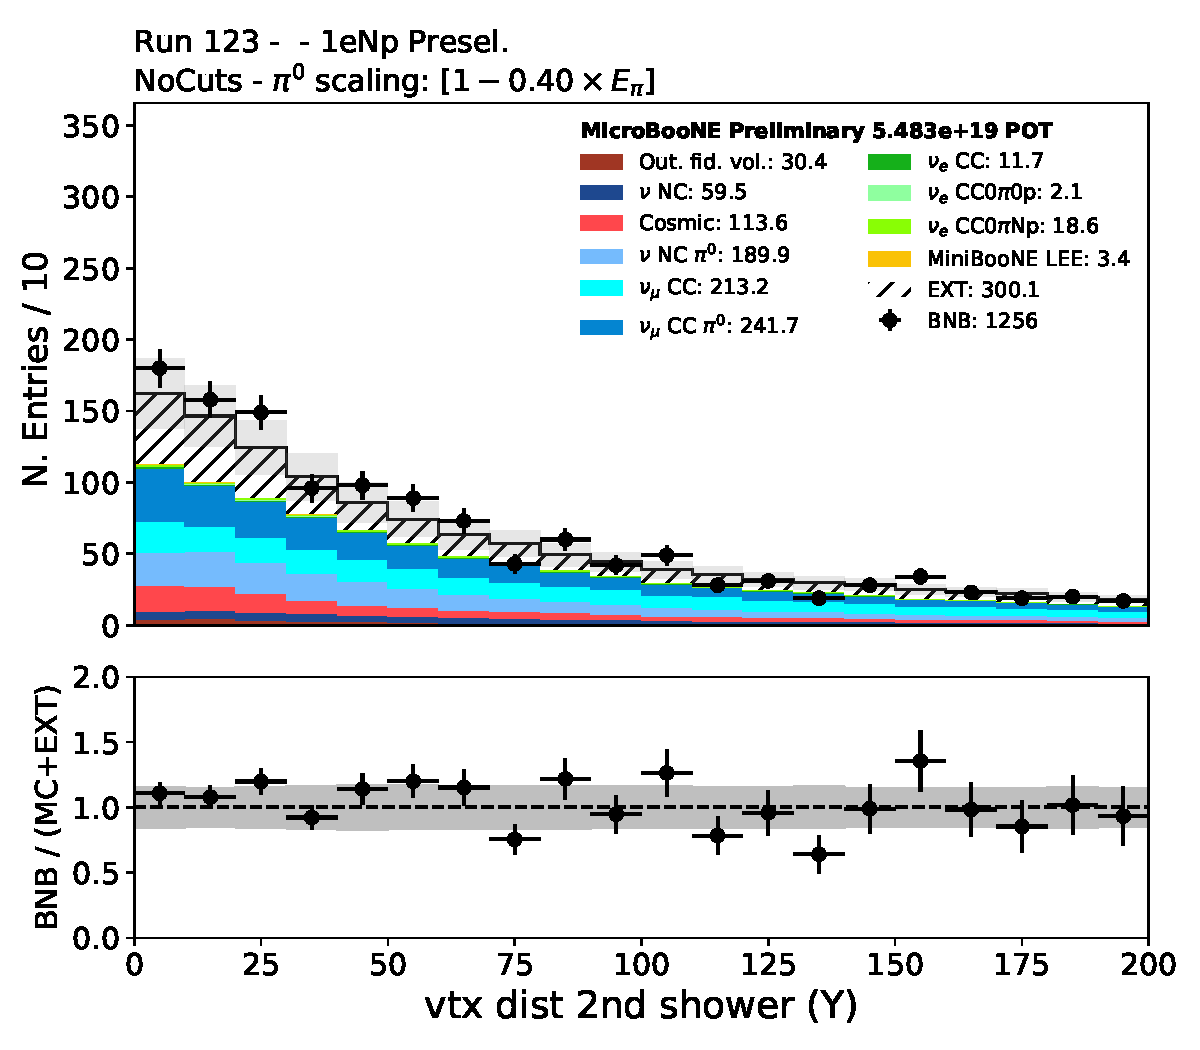
\includegraphics[width=1.00\textwidth]{1eNp/dataMCRun13/secondshower_Y_vtxdist.pdf}
    \caption{\label{fig:1eNp:dataMCRun1:secondshower_Y_vtxdist} secondshower\_Y\_vtxdist }
    \end{subfigure}
    \begin{subfigure}[b]{0.3\textwidth}
    \centering
    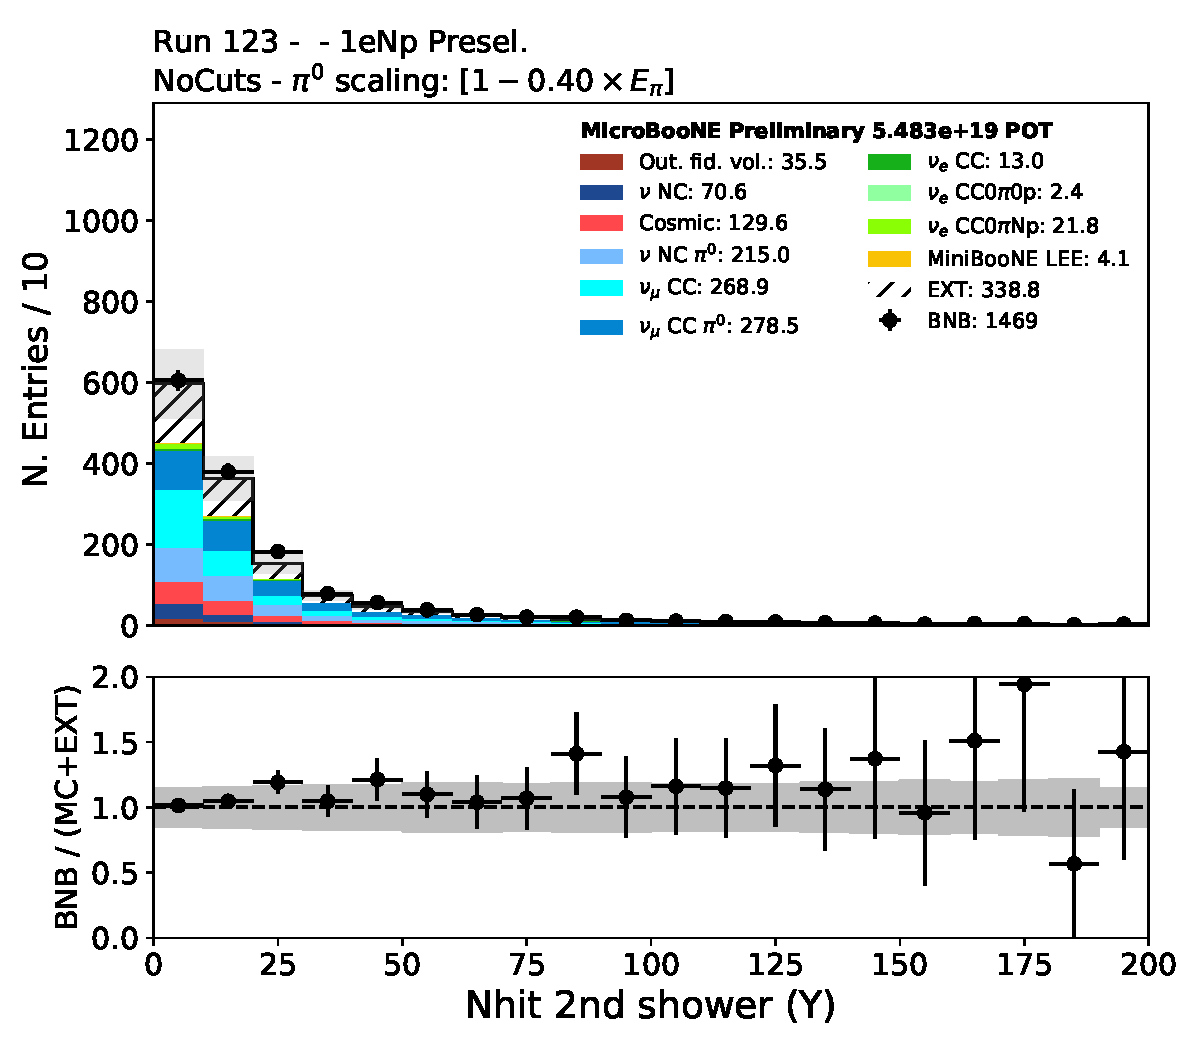
\includegraphics[width=1.00\textwidth]{1eNp/dataMCRun13/secondshower_Y_nhit.pdf}
    \caption{\label{fig:1eNp:dataMCRun1:secondshower_Y_nhit} secondshower\_Y\_nhit }
    \end{subfigure}
\caption{\label{fig:1eNp:dataMCRun1:pi01}Data-MC comparison in the Run1 open data after the \npsel preselection.}
\end{center}
\end{figure}

\begin{figure}[H] 
\begin{center}
    \begin{subfigure}[b]{0.3\textwidth}
    \centering
    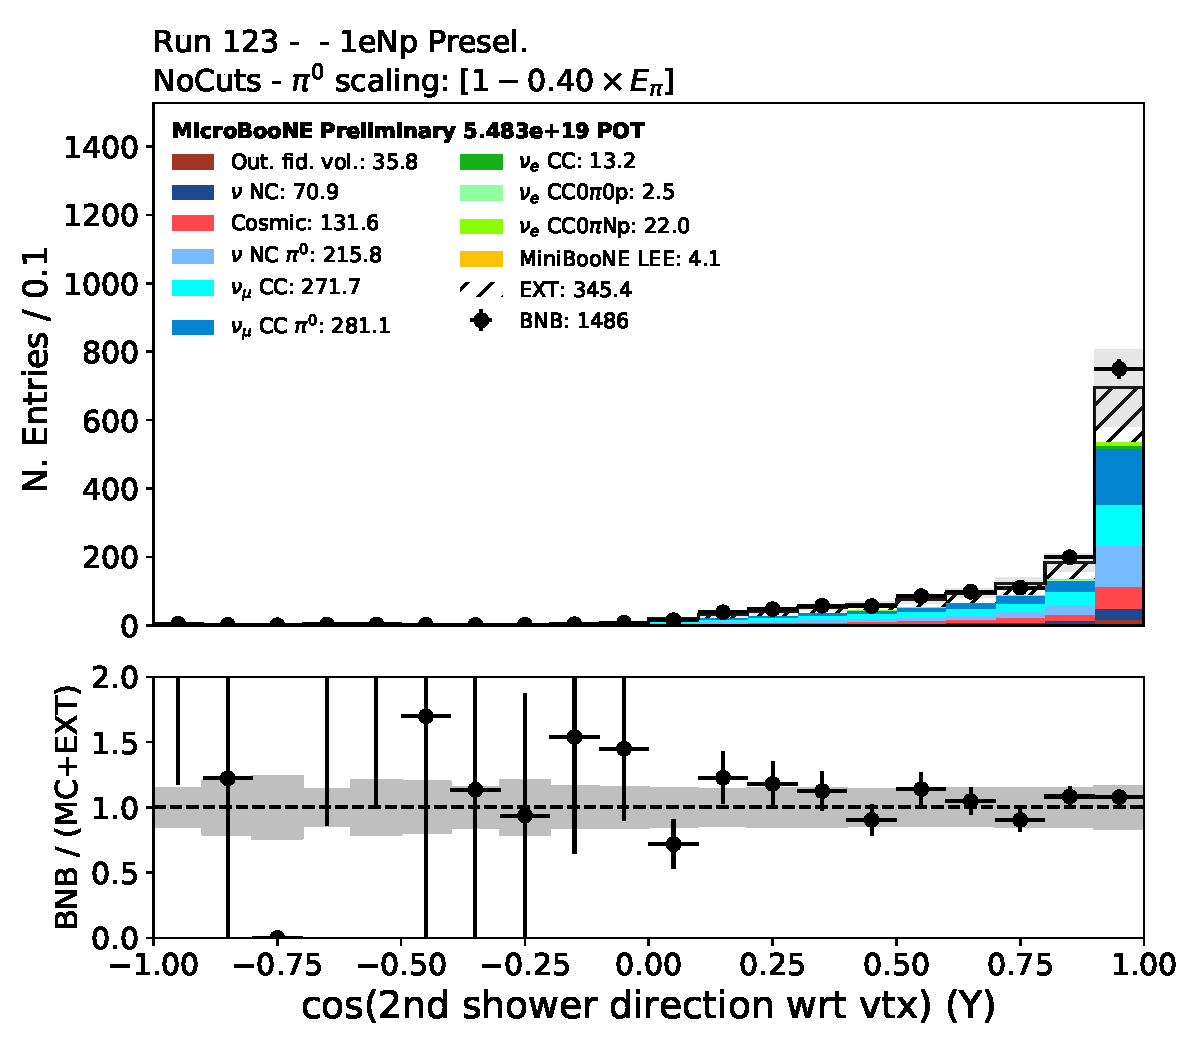
\includegraphics[width=1.00\textwidth]{1eNp/dataMCRun13/secondshower_Y_dot.pdf}
    \caption{\label{fig:1eNp:dataMCRun1:secondshower_Y_dot} secondshower\_Y\_dot }
    \end{subfigure}
    \begin{subfigure}[b]{0.3\textwidth}
    \centering
    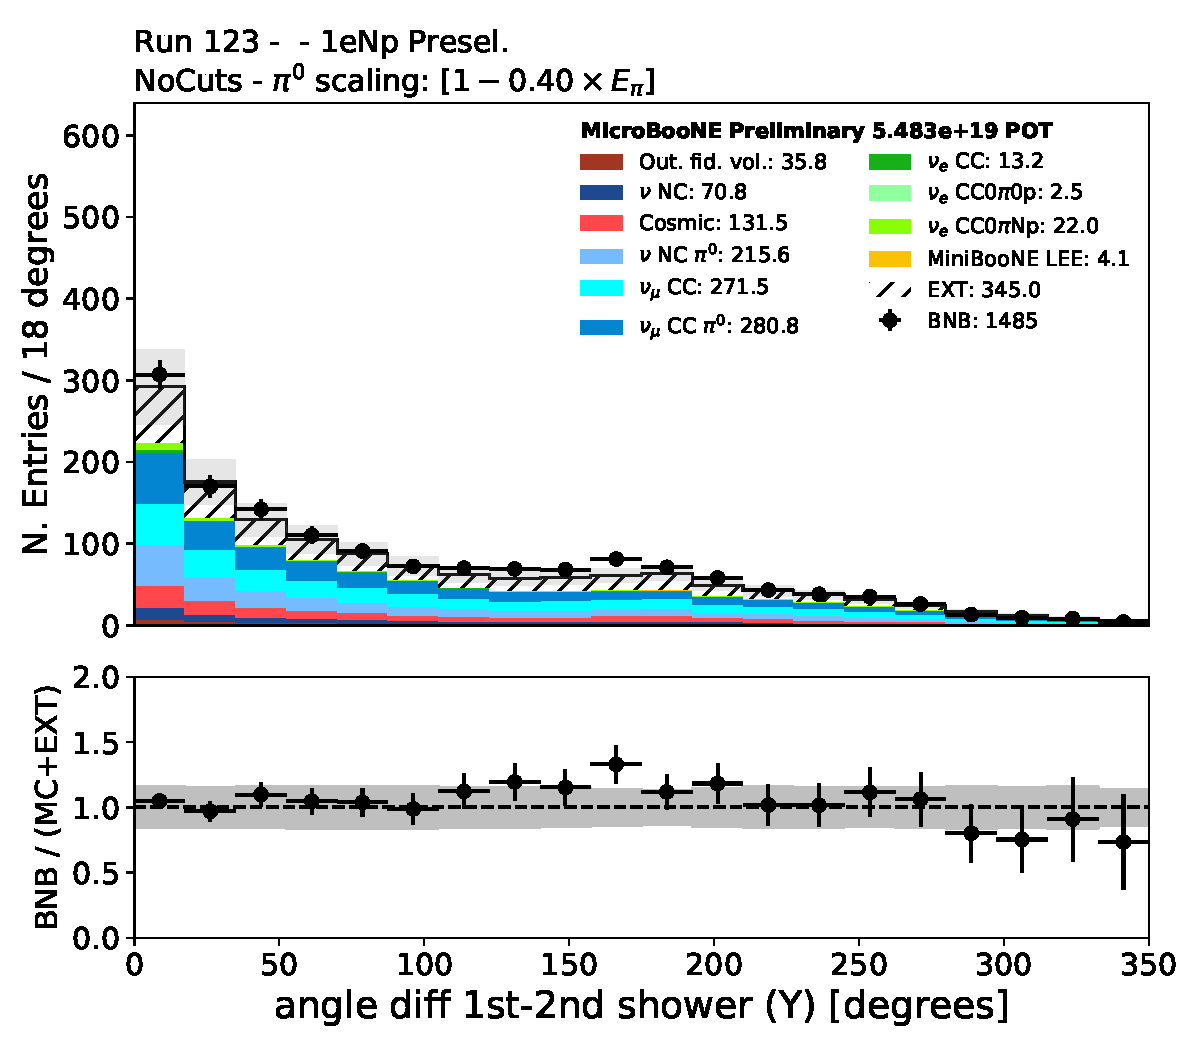
\includegraphics[width=1.00\textwidth]{1eNp/dataMCRun13/anglediff_Y.pdf}
    \caption{\label{fig:1eNp:dataMCRun1:anglediff_Y} anglediff\_Y }
    \end{subfigure}
    \begin{subfigure}[b]{0.3\textwidth}
    \centering
    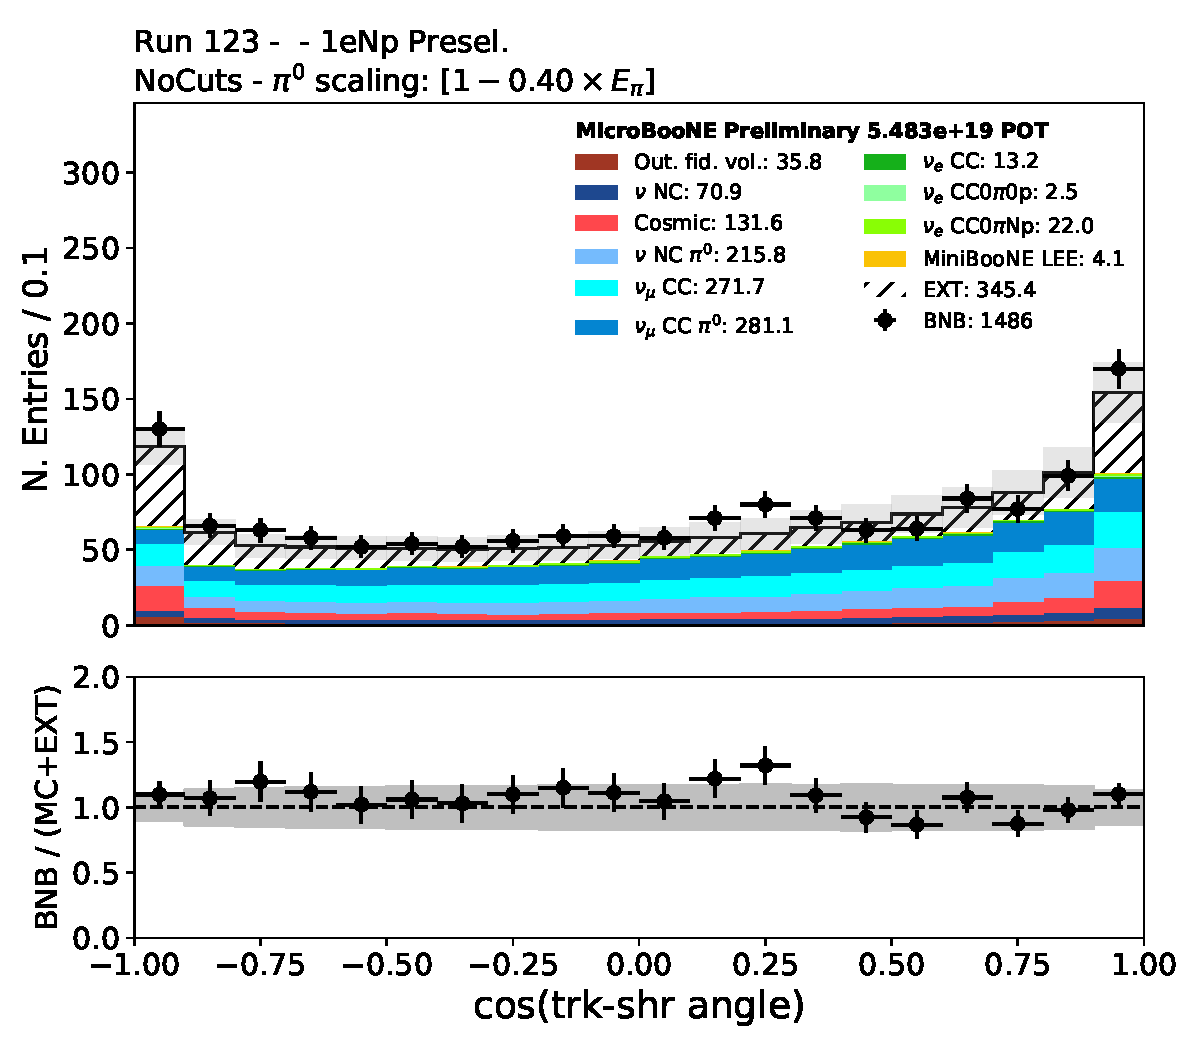
\includegraphics[width=1.00\textwidth]{1eNp/dataMCRun13/tksh_angle.pdf}
    \caption{\label{fig:1eNp:dataMCRun1:tksh_angle} tksh\_angle }
    \end{subfigure}
\caption{\label{fig:1eNp:dataMCRun1:pi02}Data-MC comparison in the Run1 open data after the \npsel preselection.}
\end{center}
\end{figure}
\clearpage
\newpage